\subsection{Interface}
\label{sect:maw_interface}

The home screen of \mawapp displays a list of pathways that the user can choose
from to view a graph. This screen is shown in figure
\ref{fig:maw_screenshot_list}. It also contains a brief explanation of the
PathCase database and instructions for using \mawapp. The button in the bottom
left corner activates the SMDA tool, described in section \ref{sect:smda}.

\begin{figure}[htbp]
    \center{
        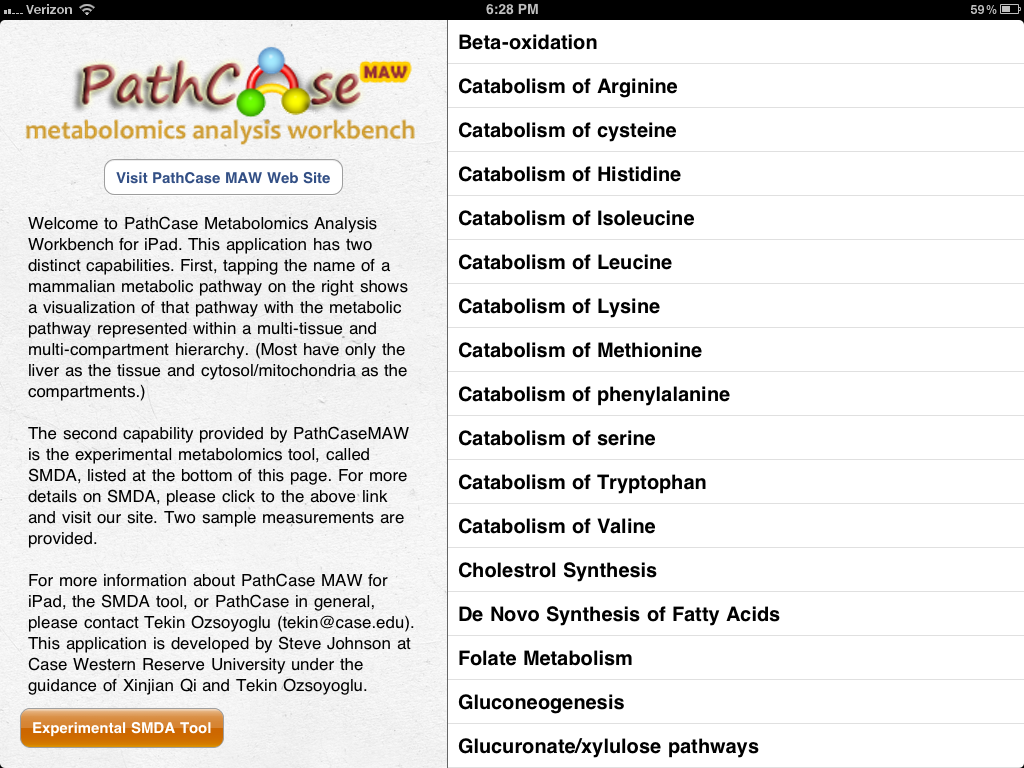
\includegraphics[width=4.5in]{maw/figures/screenshot_list}}
    \caption{\label{fig:maw_screenshot_list} List of pathways on the main screen
    of \mawapp}
\end{figure}

\begin{figure}[hbtp]
    \center{
        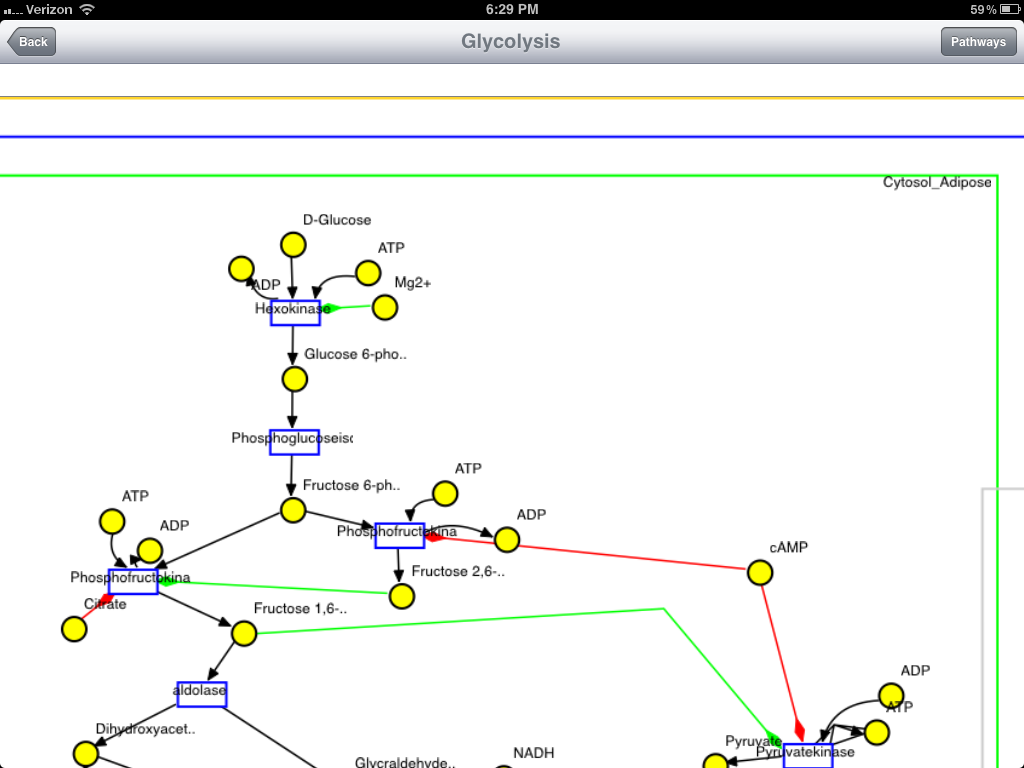
\includegraphics[width=4.5in]{maw/figures/screenshot_glycolysis}}
    \caption{\label{fig:maw_screenshot_pathway} Compartment-aware visualization
    of Glycolysis}
\end{figure}

After selecting a pathway by tapping a row in the list, the user enters the
pathway visualization. In this screen, they can drag across the screen with one
finger to move the view. They can use two fingers in a pinching motion to zoom
in or out. The view for glycolysis is shown in figure
\ref{fig:maw_screenshot_pathway}.

The pathway visualization consists of several components. The most important are
the nodes in the graph. The rectangular nodes represent reactions. The rest of
the nodes represent metabolites. The edges represent relationships such as
product, substrate, cofactor, or inhibitor. The rectangular outlines around
sections of the graph represent the compartment that the pathway is classified
under.

In figure \ref{fig:maw_screenshot_pathway}, Glycolysis is displayed in two
different compartments: $Organs \rightarrow Blood \rightarrow Cytosol\_Adipose$
and $Organs \rightarrow Blood \rightarrow Cytosol\_Liver$. These compartments
are shown using nested rectangles with text labels in the upper right corner.

\begin{figure}[hbtp]
    \center{
        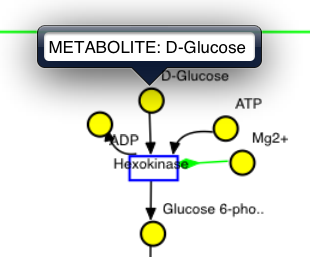
\includegraphics[width=3in]{maw/figures/screenshot_glycolysis_popover}}
    \caption{\label{fig:maw_screenshot_popover} Tapping a node displays a
    popover with the node's full name}
\end{figure}

When a node is tapped, a popover appears with the full name of the object
represented by the nodes, as well as any relevant relationships or other
information. Figure \ref{fig:maw_screenshot_popover} demonstrates this behavior.
